\documentclass{article}
\usepackage[margin=1.25in]{geometry}
\usepackage{amsmath, amssymb, setspace, enumerate, enumitem}
\usepackage{setspace}
\usepackage{graphicx}
\onehalfspacing

\begin{document}

    \begin{enumerate}
        \item \begin{enumerate}[label=(\alph*)]
            \item linear regression with pocket\\
                training:\\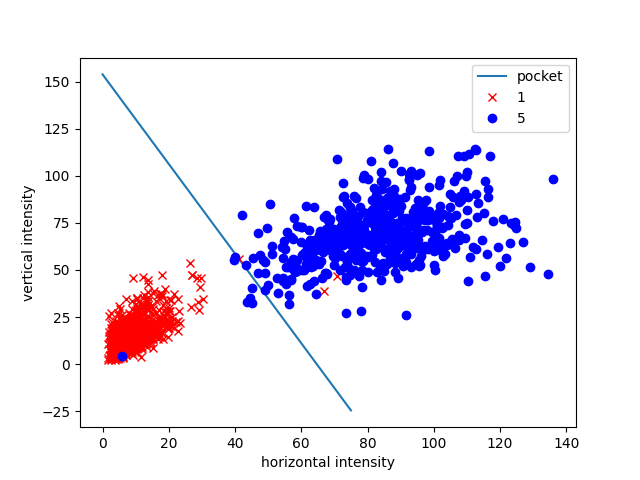
\includegraphics[scale=0.5]{images/linearpocket.png}\\
                test:\\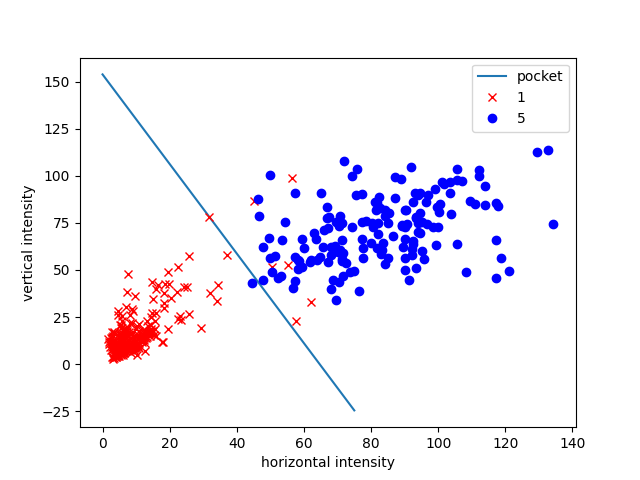
\includegraphics[scale=0.5]{images/linearpockettest.png}\\[0.25in]
                \textbf{NOTE: my logistic regression functions didn't work :(, I followed the algorithm on page 95 of the book. I still included it to show progress, the attempted code file is submitted as well.}\\
                logistic regression with gd\\
                training:\\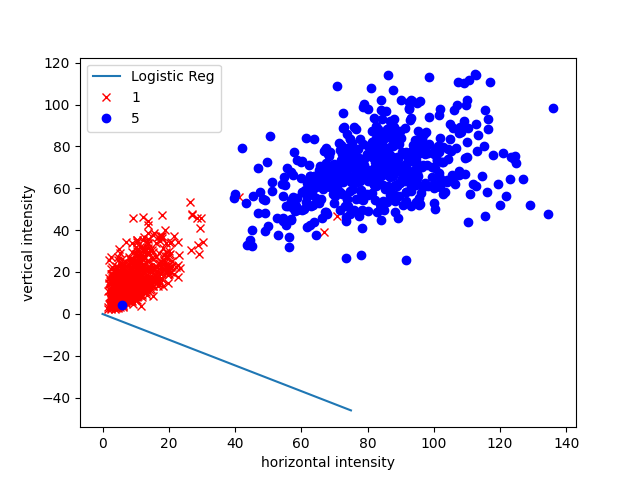
\includegraphics[scale=0.5]{images/logisticReg.png}\\
                test:\\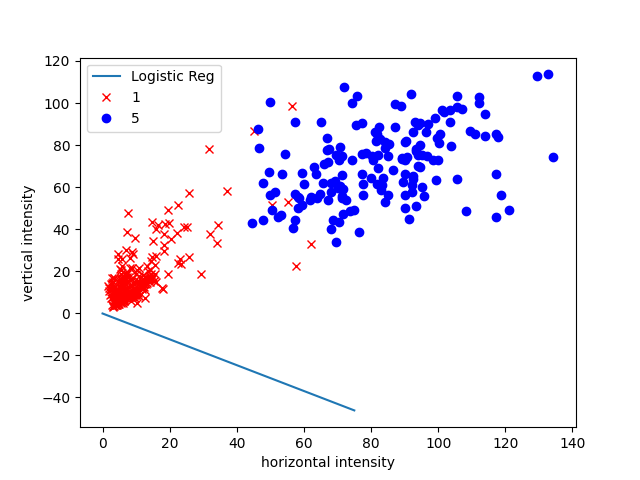
\includegraphics[scale=0.5]{images/logisticRegtest.png}\\[0.25in]
            \item linear regression with pocket\\
                $E_{in} = 0.0058$, $E_{test} = 0.0165$\\[0.25in]
                logistic regression with gradient descent\\
                $E_{in} = 0.3562$, $E_{test} = 0.3774$\\[0.25in]
            \item Since my algorithm for logistic regression did not work, I will assume linear regression w/ pocket is the method with the minimum $E_{in}$. With approximation \& generalization, we have derived the following formula:
                \begin{align*}
                    E_{out}(g) \leq E_{in}(g) + \sqrt{\frac{8}{N}\ln{\frac{4m_H(N)}{\delta}}}
                \end{align*}
                where our error bar
                \begin{align*}
                    \Omega = \sqrt{\frac{8}{N}\ln{\frac{4m_H(N)}{\delta}}}
                \end{align*}
                We can plug in $N = 1561$, $\delta = 0.05$, $d_{vc}$ = 3, $m_H(1561) = (2(1561))^{3} + 1$, and $E_in = 0.0058$, then we derive the equation:
                \begin{align*}
                    E_{out}(g) &\leq 0.0058 + \sqrt{\frac{8}{1561}\ln{\frac{4((2(1561))^3+1)}{0.05}}}\\
                    &\leq 0.388
                \end{align*}
            \item For our testing data, we can use (2.1)
                \begin{align*}
                    E_{out}(g) \leq E_{test}(g) + \sqrt{\frac{1}{2N}\ln{\frac{2M}{\delta}}}
                \end{align*}
                Where $N = 424$, $\delta = 0.05$, $M = 1$
                \begin{align*}
                    E_{out}(g) &\leq 0.0118 + \sqrt{\frac{1}{2(424)}\ln{\frac{2}{0.05}}}\\
                    &\leq 0.0824
                \end{align*}
            \item
            \begin{enumerate}[label=(\alph*)]
                \item linear regression w/ pocket:\\
                    training:\\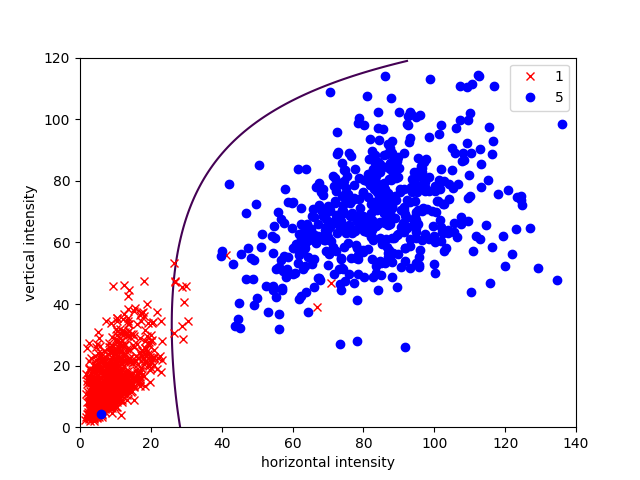
\includegraphics[scale=0.5]{images/linearpocket3rd.png}\\
                    test:\\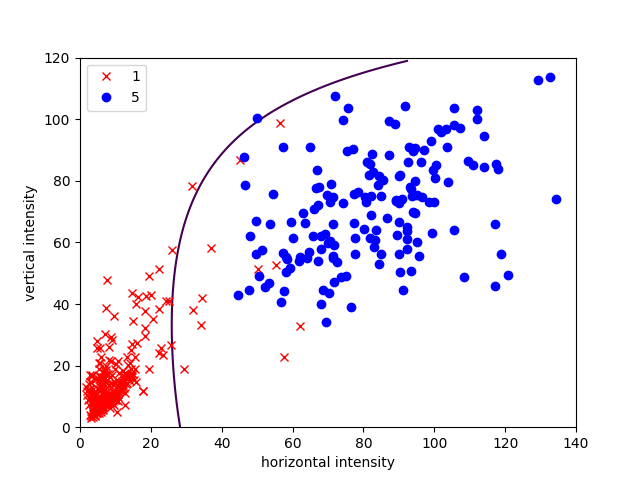
\includegraphics[scale=0.5]{images/linearpocket3rdtest.png}\\
                    \textbf{As mentioned above, algorithms for logistic regression didn't work despite following the code in page 95 :(, attempt is shown in code, so no plot was created for logistic regression}
                \item for linear regression w/ pocket: $E_{in} = 0.0032$, $E_{test} = 0.0212$
                \item We can reuse the formula from above:
                    \begin{align*}
                        E_{out}(g) \leq E_{in}(g) + \sqrt{\frac{8}{N}\ln{\frac{4m_H(N)}{\delta}}}
                    \end{align*}
                    We can plug in $N = 1561$, $\delta = 0.05$, $d_{vc}$ = 10, $m_H(1561) = (2(1561))^{10} + 1$, and $E_in = 0.0058$, then we derive the equation:
                    \begin{align*}
                        E_{out}(g) &\leq 0.0058 + \sqrt{\frac{8}{1561}\ln{\frac{4((2(1561))^{10}+1)}{0.05}}}\\
                        &\leq 0.665
                    \end{align*}
                \item We can reuse the formula from above:
                    \begin{align*}
                        E_{out}(g) \leq E_{test}(g) + \sqrt{\frac{1}{2N}\ln{\frac{2M}{\delta}}}
                    \end{align*}
                    Where $N = 424$, $\delta = 0.05$, $M = 1$
                    \begin{align*}
                        E_{out}(g) &\leq 0.0212 + \sqrt{\frac{1}{2(424)}\ln{\frac{2}{0.05}}}\\
                        &\leq 0.08716
                    \end{align*}
            \end{enumerate}
            \item Linear model without the 3rd order polynomial transform. It may seem counter-intuitive that, despite a lower $E_{in}$ and $E_{test}$, we don't choose the one with 3rd order transform. As discussed in lecture, when a problem gets more complex, our solution becomes simpler, this means a lower $d_{vc}$, we can't assume the size of the dataset that the customer will provide, but if we assume that it is large, then we want the simplest curve possible, which we obtain from the linear model without the 3rd order polynomial transform.
        \end{enumerate}
        \item \begin{enumerate}[label=(\alph*)]
            \item When the learning rate was set to 0.01, there was a stable decline in the function, when the learning rate was raised to 0.1, it became scattered. This is due to the function jumping around, trying to find the local minimum, but the learning rate is too high, so it's jumping more than it should.
            \item Learning rate set to 0.01:\\
                \begin{tabular}{ c c c c c }
                    x start & y start & x min & y min & min value\\
                    0.1 & 0.1 & 0.24380496936478335 & -0.23792582148617658 & -1.8200785415471565\\
                    1 & 1 & 1.2180703009052047 & 0.7128119503387537 & 0.5932693743258357\\
                    -0.5 & -0.5 & -0.731377460409601 & -0.23785536290147238 & -1.332481062330978\\
                    -1 & -1 & -1.2180703009052047 & -0.7128119503387537 & 0.5932693743258357\\
                \end{tabular}

                Learning rate set to 0.1:\\
            \begin{tabular}{c c c c c}
                x start & y start & x min & y min & min value\\
                0.1 & 0.1 & 0.23624085417279922 & 0.2292203653889578 & -1.6452216178404533\\
                1 & 1 & 0.5638448167590557 & -0.03503546573154889 & -1.6997441668889812\\
                -0.5 & -0.5 & -0.01859951030800544 & 0.4009863778325866 & -1.3964666430345036\\
                -1 & -1 & -0.5638448167590557 & 0.03503546573154889 & -1.6997441668889812\\
            \end{tabular}
        \end{enumerate}

        \item \begin{enumerate}[label=(\alph*)]
            \item cost(accept) (+1) = $0 \times correct + c_a \times incorrect = c_a \times incorrect = (1 - g(x))c_a$\\
                cost(reject) (-1) = $c_r \times correct + 0 \times incorrect = c_r \times correct = g(x)c_r$
            \item We accept when $g(x) \geq k$, so 
                \begin{align*}
                    (1 - g(x))c_a &\geq g(x)c_r \\
                    c_a - c_ag(x) &\geq g(x)c_r \\
                    -c_ag(x) - g(x)c_r &\geq -c_a\\
                    g(x)(-c_a - c_r) &\geq -c_a \\
                    g(x) &\geq \frac{-c_a}{-c_a - c_r}\\
                    g(x) &\geq \frac{c_a}{c_a + c_r}
                \end{align*}
                If we let
                \begin{align*}
                    k = \frac{c_a}{c_a + c_r}
                \end{align*}
                Then we have fulfilled our accepting condition $g(x) \geq k$
            \item Supermarket: $c_a = 1$ and $c_r = 10$
                \begin{align*}
                    k = \frac{1}{1 + 10} = 0.09090909
                \end{align*}
                CIA: $c_a = 1000$ and $c_r = 1$
                \begin{align*}
                    k = \frac{1000}{1000 + 1} = 0.999000999
                \end{align*}
                Intuitively, the CIA would have a higher threshhold because the cost of accepting a person's fingerprints when it should've been rejecting is high. Whereas the supermarket, if you accept false accept, it is not a big deal and thus have low cost.
        \end{enumerate}
    \end{enumerate}

\end{document}